\section{Globale Testfälle}
Es werden die Fälle anhand von UseCase visualisiert, welche bei der Interaktion von Produkt externen Einflüssen passieren.
\\
\paragraph{Akteure}\mbox{}\\
\begin{figure}[H]
	\centering
	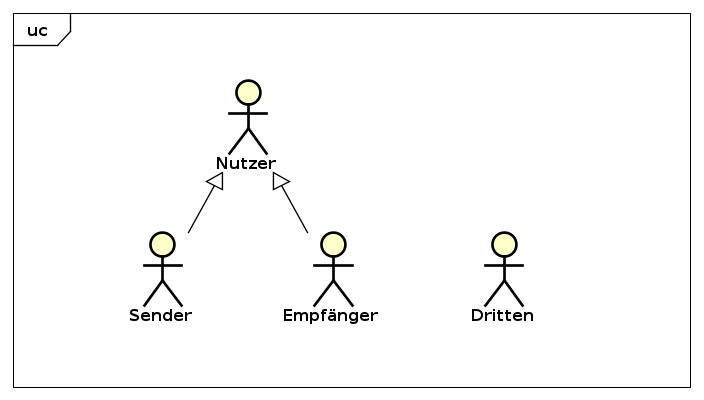
\includegraphics[width= 0.9\linewidth]{diagramms/useCase/akteure.png}
	\caption{Akteure}
\end{figure}
In der Abbildung 22, sind alle Akteure die in den folgenden Use-Case-Diagrammen vorkommen abgebildet. Hierbei gibt es einen Nutzer welcher sowohl ein Sender als auch ein Empfänger sein kann. Darüber hinaus gibt es Dritte welche in den Use-Cases mögliche Bedrohungen darstellt.
\newpage
\paragraph{Datentransfer}\mbox{}\\
\begin{figure}[H]
	\centering
	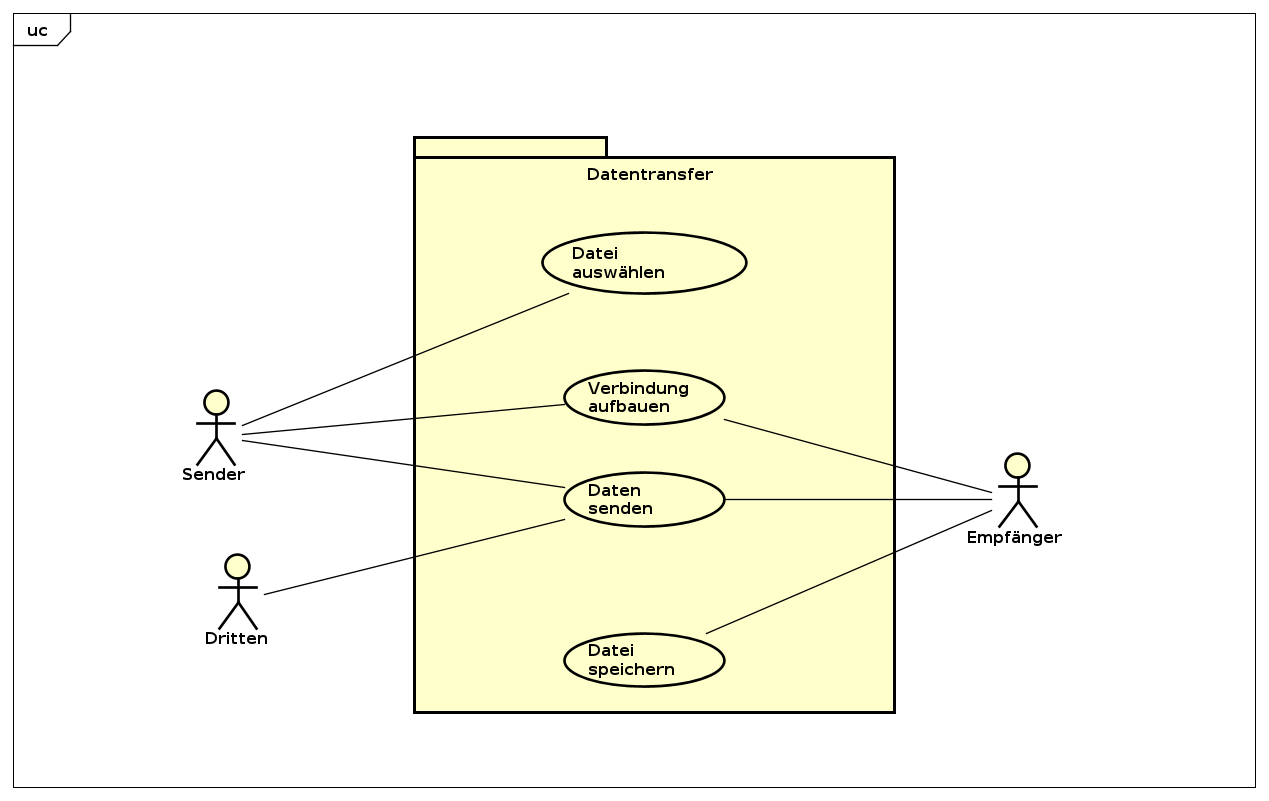
\includegraphics[width= 0.9\linewidth]{diagramms/useCase/datentransfer.png}
	\caption{Datentransfer}
\end{figure}
In der Abbildung wird der Grobe Datentransfer beschrieben. Hierbei ist jedes Use-Case auf den folgenden Seiten genauer vorgeführt und erklärt.
\newpage
\paragraph{Datei auswählen}\mbox{}\\
\begin{figure}[H]
	\centering
	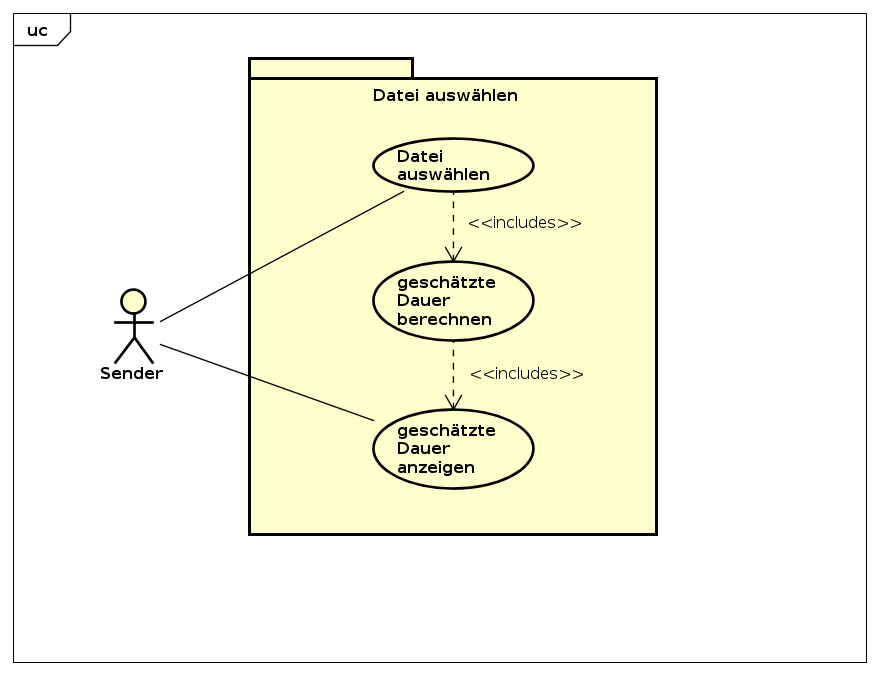
\includegraphics[width= 0.9\linewidth]{diagramms/useCase/datei_auswaehlen.png}
	\caption{Datei auswählen}
\end{figure}
Wenn der Sender auf den, im Mockup gezeigten, Knopf drückt öffnet sich der File Explorer wo man dann eine Datei auswählen kann. Nachdem die Datei ausgewählt wurde wird die geschätzte Dauer, welche für die Übertragung benötigt wird, berechnet und angezeigt.
\newpage
\paragraph{Verbindung aufbauen}\mbox{}\\
\begin{figure}[H]
	\centering
	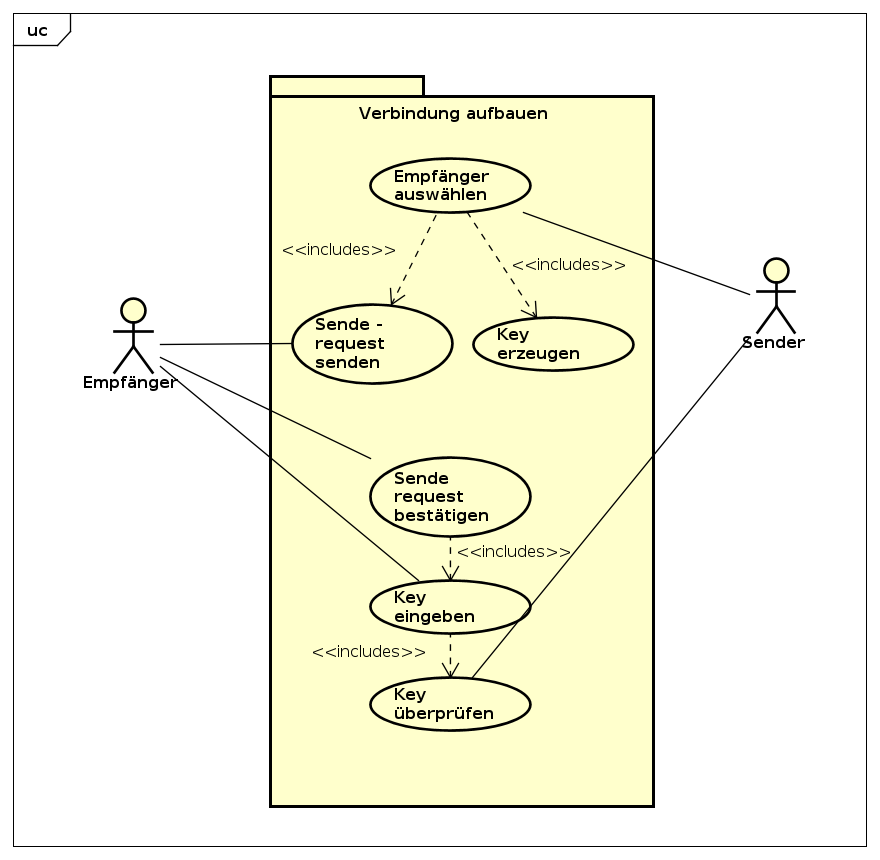
\includegraphics[width= 0.9\linewidth]{diagramms/useCase/verbindung_aufbauen.png}
	\caption{Verbindung aufbauen}
\end{figure}
Wenn der Sender nun die Datei ausgewählt hat muss er einen Empfänger auswählen. Nachdem er dies getan hat, wird ein Key erzeugt und eine Sende-Request gesendet. Der Empfänger der Datei bestätigt diese und muss danach den Key eingeben. Nach der Eingabe wird geprüft ob der Key mit dem vom Sender übereinstimmt.
\newpage
\paragraph{Daten senden}\mbox{}\\
\begin{figure}[H]
	\centering
	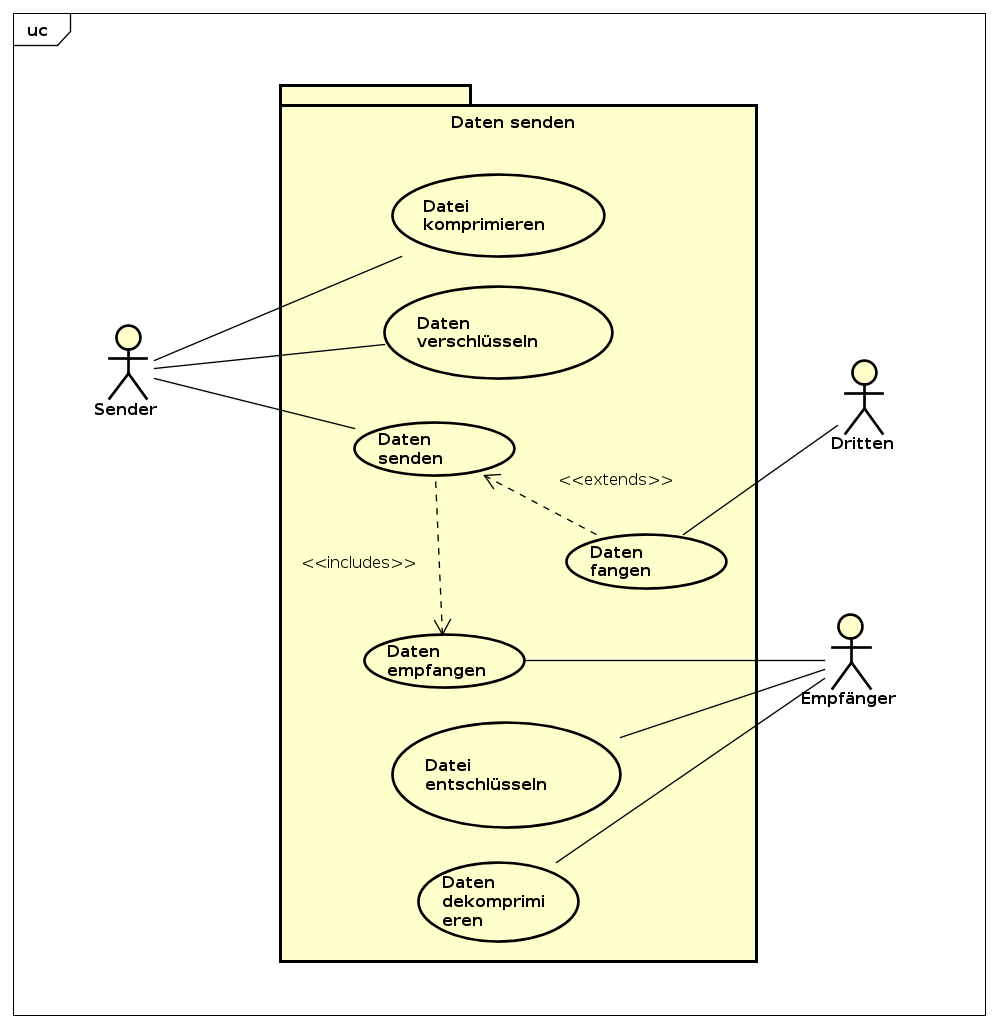
\includegraphics[width= 0.9\linewidth]{diagramms/useCase/daten_senden.png}
	\caption{Daten senden}
\end{figure}
Nachdem der Empfänger ausgewählt und der Key bestätigt wurde, wird Datei komprimiert und anschließend verschlüsselt. Wenn diese Schritte erfolgreich durchlaufen werden, wird die Datei versendet. Nun könnten die Dritten versuchen die Daten abzufangen. Falls dieser Versuch fehlschlägt oder gar nicht erst zustande erhält  der Empfänger die Datei und kann sie entschlüsseln und dekomprimieren.
\newpage
\paragraph{Datei speichern}\mbox{}\\
\begin{figure}[H]
	\centering
	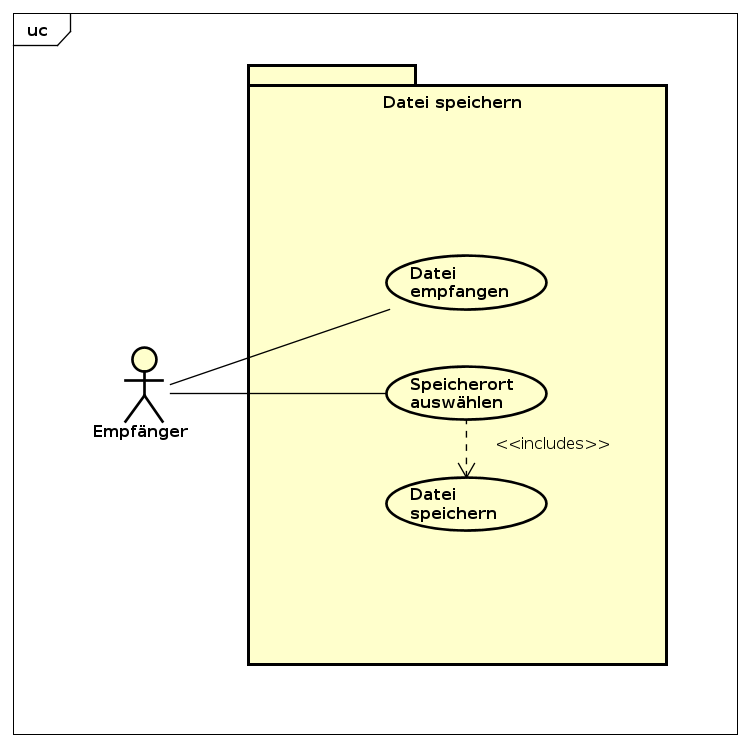
\includegraphics[width= 0.9\linewidth]{diagramms/useCase/datei_speichern.png}
	\caption{Datei speichern}
\end{figure}
Wenn der Empfänger die Datei erhält muss er einen Speicherort für sie wählen. Nachdem dieser gewählt wurde wird die Datei gespeichert.